%%%%%%%%%%%%%%%%%%%%%%%%%%%%%%%%%%%%%%%%%
% Jacobs Landscape Poster
% LaTeX Template
% Version 1.1 (14/06/14)
%
% Created by:
% Computational Physics and Biophysics Group, Jacobs University
% https://teamwork.jacobs-university.de:8443/confluence/display/CoPandBiG/LaTeX+Poster
% 
% Further modified by:
% Nathaniel Johnston (nathaniel@njohnston.ca)
%
% This template has been downloaded from:
% http://www.LaTeXTemplates.com
%
% License:
% CC BY-NC-SA 3.0 (http://creativecommons.org/licenses/by-nc-sa/3.0/)
%
%%%%%%%%%%%%%%%%%%%%%%%%%%%%%%%%%%%%%%%%%

%----------------------------------------------------------------------------------------
%	PACKAGES AND OTHER DOCUMENT CONFIGURATIONS
%----------------------------------------------------------------------------------------

\documentclass[final]{beamer}

\usepackage[scale=1.24]{beamerposter} % Use the beamerposter package for laying out the poster

\usetheme{confposter} % Use the confposter theme supplied with this template

\setbeamercolor{block title}{fg=ngreen,bg=white} % Colors of the block titles
\setbeamercolor{block body}{fg=black,bg=white} % Colors of the body of blocks
\setbeamercolor{block alerted title}{fg=white,bg=dblue!70} % Colors of the highlighted block titles
\setbeamercolor{block alerted body}{fg=black,bg=dblue!10} % Colors of the body of highlighted blocks
% Many more colors are available for use in beamerthemeconfposter.sty

%-----------------------------------------------------------
% Define the column widths and overall poster size
% To set effective sepwid, onecolwid and twocolwid values, first choose how many columns you want and how much separation you want between columns
% In this template, the separation width chosen is 0.024 of the paper width and a 4-column layout
% onecolwid should therefore be (1-(# of columns+1)*sepwid)/# of columns e.g. (1-(4+1)*0.024)/4 = 0.22
% Set twocolwid to be (2*onecolwid)+sepwid = 0.464
% Set threecolwid to be (3*onecolwid)+2*sepwid = 0.708

\newlength{\sepwid}
\newlength{\onecolwid}
\newlength{\twocolwid}
\newlength{\threecolwid}
\setlength{\paperwidth}{48in} % A0 width: 46.8in
\setlength{\paperheight}{36in} % A0 height: 33.1in
\setlength{\sepwid}{0.024\paperwidth} % Separation width (white space) between columns
\setlength{\onecolwid}{0.22\paperwidth} % Width of one column
\setlength{\twocolwid}{0.464\paperwidth} % Width of two columns
\setlength{\threecolwid}{0.708\paperwidth} % Width of three columns
\setlength{\topmargin}{-0.5in} % Reduce the top margin size
%-----------------------------------------------------------

\usepackage{graphicx}  % Required for including images

\usepackage{booktabs} % Top and bottom rules for tables

%----------------------------------------------------------------------------------------
%	TITLE SECTION 
%----------------------------------------------------------------------------------------

\title{BachBot: Deep generative modeling of Bach chorales} % Poster title


\author[shortname]{Feynman Liang\inst{1}, Marcin Tomczak\inst{1}, Matt
Johnson\inst{2}, Mark Gotham\inst{3}, Jamie Shotten\inst{2}, \and Bill
Byrne\inst{1}}

\institute[shortinst]{\inst{1} Cambridge University Engineering Department,
  \inst{2} Microsoft Research Cambridge, \and
\inst{3} Faculty of Music, University of Cambridge}

%----------------------------------------------------------------------------------------

\begin{document}

\addtobeamertemplate{block end}{}{\vspace*{2ex}} % White space under blocks
\addtobeamertemplate{block alerted end}{}{\vspace*{2ex}} % White space under highlighted (alert) blocks

\setlength{\belowcaptionskip}{2ex} % White space under figures
\setlength\belowdisplayshortskip{2ex} % White space under equations

\begin{frame}[t] % The whole poster is enclosed in one beamer frame

\begin{columns}[t] % The whole poster consists of three major columns, the second of which is split into two columns twice - the [t] option aligns each column's content to the top

\begin{column}{\sepwid}\end{column} % Empty spacer column

\begin{column}{\onecolwid} % The first column

%----------------------------------------------------------------------------------------
%	OBJECTIVES
%----------------------------------------------------------------------------------------

\begin{alertblock}{Objectives}

  The goal of BachBot is to generate 4-part Baroque chorales in the stype of
  Johann Sebastian Bach. We interpret this as sampling random chorales from a
  generative probabilistic model of Bach chorales and identify four discrete
  objectives:
\begin{itemize}
  \item \textbf{Melody modeling}: Marginal distribution over univariate Soprano melody sequences
  \item \textbf{Melody harmonization}: Conditional distribution over
    multivariate (Alto, Tenor, and Bass) harmony parts given fixed Sporano
    melody
  \item \textbf{One-pass polyphonic generation}: Sequentially modeling of all parts jointly
  \item \textbf{Applications in music analysis}: What would Bach do? Enhance ``Bach-ness'' of inputs.
\end{itemize}

\end{alertblock}

%----------------------------------------------------------------------------------------
%	Background
%----------------------------------------------------------------------------------------

\begin{block}{Background}
  Music is quantized to the nearest 16th beat (the smallest metric interval
  occuring in Bach chorales) and quantized to the twelve note chromatic scale
  used in Western music. We define two equivalent representations for music:
  \begin{itemize}
    \item The \textbf{per-parts tuples} representation consists of four collections (one for
      each voice) of note/rest and duration tuples. Note that durations between adjacent
      tuples are non-uniform.
    \item The \textbf{per-parts roll} consists of a categorical array $X_{p,t} \in V$
      denoting the note played by part $p \in \{S,A,T,B\}$ at time $t \in \{1,2,\cdots,T\}$
      To distinguish notes held from previous times from notes articulated at the current
      time, $Y_{p,t} \in \{0,1\}$ indicates if the note is articulated at time $t$.
    \item The \textbf{piano roll} is like the per-parts roll except $X_{n,t} \in \{0,1\}$
      denotes if note $n$ is played at time $t$. Note that this definition precludes
      two parts playing the same note.
  \end{itemize}

\end{block}

%----------------------------------------------------------------------------------------

\end{column} % End of the first column

\begin{column}{\sepwid}\end{column} % Empty spacer column

\begin{column}{\twocolwid} % Begin a column which is two columns wide (column 2)

\begin{columns}[t,totalwidth=\twocolwid] % Split up the two columns wide column

\begin{column}{\onecolwid}\vspace{-.6in} % The first column within column 2 (column 2.1)

%----------------------------------------------------------------------------------------
%	MELODY
%----------------------------------------------------------------------------------------

\begin{block}{Melody Modeling}
  \begin{itemize}
    \item Given initial seed, generate melody sequence
    \item Baseline: $N$-gram language model perplexity
    \item Experiments:
      \begin{itemize}
        \item RNN, LSTM, and GRU architectures
        \item Word level vs note level features, augmentation with expert crafted features
        \item Constant (roll representation) or varying timestep (tuple representation) per input
      \end{itemize}
  \end{itemize}
\end{block}

\begin{figure}
  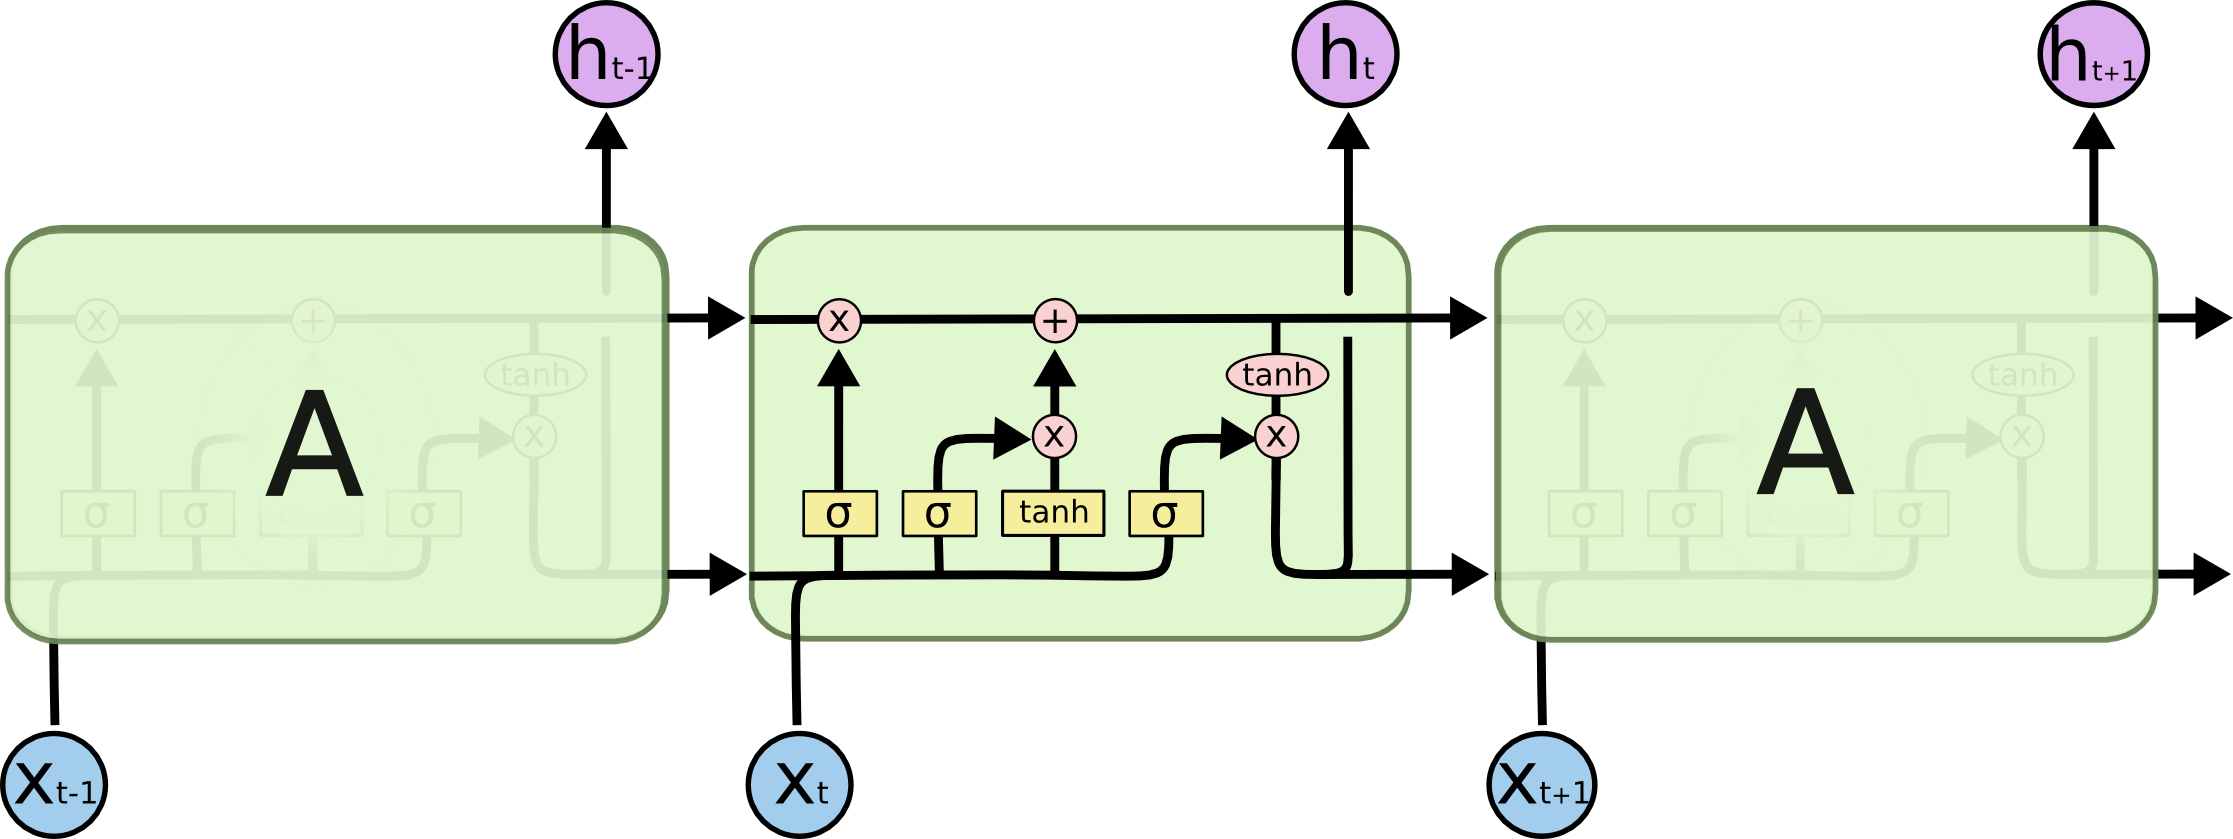
\includegraphics[width=0.8\linewidth]{LSTM3-chain.png}
  \caption{Inside of an LSTM cell\cite{DBLP:conf/asru/2013}}
\end{figure}

%----------------------------------------------------------------------------------------

\end{column} % End of column 2.1

\begin{column}{\onecolwid}\vspace{-.6in} % The second column within column 2 (column 2.2)

%----------------------------------------------------------------------------------------
%	HARMONIZATION
%----------------------------------------------------------------------------------------

\begin{block}{Melody Harmonization}

  \begin{itemize}
    \item Given melody, generate the harmony parts
    \item Baseline: HMM-based system\cite{allan2005harmonising} accuracy
    \item Experiments:
      \begin{itemize}
        \item Single multivariate vs 4 independent LSTMs with MRF refinement
        \item Bi-directional LSTM
      \end{itemize}
  \end{itemize}

  \begin{figure}
    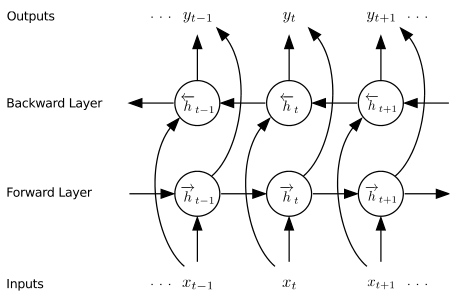
\includegraphics[width=0.8\linewidth]{bidir.png}
    \caption{Bidirectional RNN hidden states}
  \end{figure}

\end{block}

%----------------------------------------------------------------------------------------

\end{column} % End of column 2.2

\end{columns} % End of the split of column 2 - any content after this will now take up 2 columns width

%----------------------------------------------------------------------------------------
%	IMPORTANT RESULT
%----------------------------------------------------------------------------------------

% \begin{alertblock}{High Level Model}

%   Analysis tools:
%     Semantic interpretation of specificity of LSTM hidden states via plotting gate activations for inputs
%     What would Bach do? MAP estimate of next note
%     Fixing LSTM weights and optimizing the inputs

%   Training, unrolling, BPTT
%   Sampling

%   Implementation: keras, tensorflow

% \end{alertblock}

%----------------------------------------------------------------------------------------

\begin{columns}[t,totalwidth=\twocolwid] % Split up the two columns wide column again

\begin{column}{\onecolwid} % The first column within column 2 (column 2.1)

%----------------------------------------------------------------------------------------
%	One-pass polyphonic
%----------------------------------------------------------------------------------------

\begin{block}{One-pass polyphonic generation}
  \begin{itemize}
    \item Given initial seed, generate entire chorale
    \item Baseline: n/a, subjective evaluation
    \item Experiments:
      \begin{itemize}
        \item Bi-axial and grid architectures
        \item Convolutional vs recurrent dimensions
      \end{itemize}
  \end{itemize}
\end{block}

\begin{figure}
  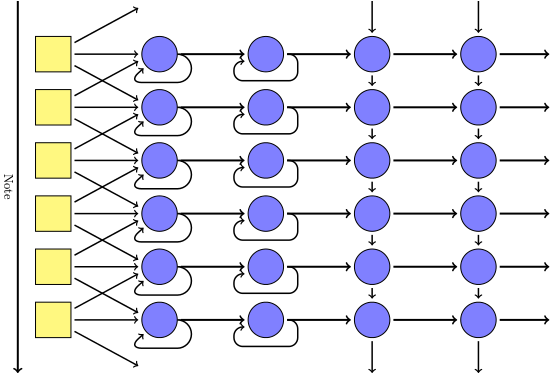
\includegraphics[width=0.95\linewidth]{biaxial.png}
  \caption{Biaxial RNN Architecture\cite{colah:lstm}}
\end{figure}

%----------------------------------------------------------------------------------------

\end{column} % End of column 2.1

\begin{column}{\onecolwid} % The second column within column 2 (column 2.2)

%----------------------------------------------------------------------------------------
%	Music Analsysis
%----------------------------------------------------------------------------------------

\begin{block}{Applications in Music Analysis}
  \begin{itemize}
    \item MAP estimation: how would Bach complete this note/melody/chorale?
    \item Interpreting hidden state activations
    \item Adversarial net: enhance ``Bach-ness'' of given input
  \end{itemize}
\end{block}

\begin{figure}
  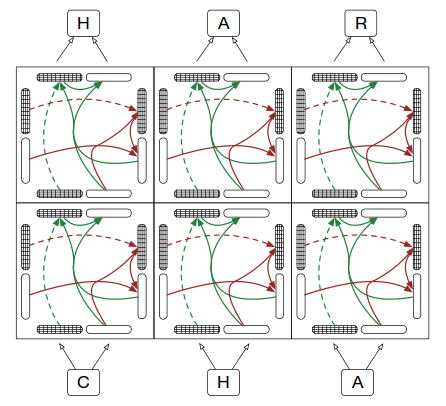
\includegraphics[width=0.95\linewidth]{grid-lstm.png}
  \caption{2D grid RNN Architecture\cite{DBLP:journals/corr/KalchbrennerDG15}}
\end{figure}

%----------------------------------------------------------------------------------------

\end{column} % End of column 2.2

\end{columns} % End of the split of column 2

\end{column} % End of the second column

\begin{column}{\sepwid}\end{column} % Empty spacer column

\begin{column}{\onecolwid} % The third column

%----------------------------------------------------------------------------------------
%	Status
%----------------------------------------------------------------------------------------

\begin{block}{Project status}

  \begin{itemize}
    \item Completed
      \begin{itemize}
        \item Preprocessing pipeline (strip markup, extract 4 parts, transpose C major/A minor) complete
        \item \texttt{torch} 2-layer LSTM melody model
        \item \texttt{keras}/\texttt{tensorflow} bi-axial LSTM modely model
      \end{itemize}
    \item Upcoming
      \begin{itemize}
        \item Get baselines for $N$-gram melody model and HMM-based harmonization \cite{allan2005harmonising}
        \item Augment feature representation with expert crafted features
        \item Investigate GRUs and vanilla RNNs for melody modeling and harmonization
        \item Implement and compare biaxial vs grid RNNs for harmonization and single pass generation
        \item Sample outputs and perform subjective evaluation using MTurk
      \end{itemize}
  \end{itemize}

\end{block}

%----------------------------------------------------------------------------------------
%	REFERENCES
%----------------------------------------------------------------------------------------

\begin{block}{References}

\nocite{*} % Insert publications even if they are not cited in the poster
\small{\bibliographystyle{unsrt}
\bibliography{sample}\vspace{0.75in}}

\end{block}

%----------------------------------------------------------------------------------------
%	ACKNOWLEDGEMENTS
%----------------------------------------------------------------------------------------

\setbeamercolor{block title}{fg=red,bg=white} % Change the block title color

\begin{block}{Acknowledgements}

\small{\rmfamily{We gratefully acknowledge the support of Microsoft Research
Cambridge with the donation of GPUs used for this research.}} \\

\end{block}

%----------------------------------------------------------------------------------------
%	CONTACT INFORMATION
%----------------------------------------------------------------------------------------

\setbeamercolor{block alerted title}{fg=black,bg=norange} % Change the alert block title colors
\setbeamercolor{block alerted body}{fg=black,bg=white} % Change the alert block body colors

\begin{alertblock}{Contact Information}

\begin{itemize}
\item \href{https://github.com/feynmanliang/bachbot}{https://github.com/feynmanliang/bachbot}
\item \href{mailto:fl350@cam.ac.uk}{fl350@cam.ac.uk}
\end{itemize}

\end{alertblock}

\begin{center}
  
\includegraphics[width=0.5\linewidth]{Engineering.png}
\end{center}

%----------------------------------------------------------------------------------------

\end{column} % End of the third column

\end{columns} % End of all the columns in the poster

\end{frame} % End of the enclosing frame

\end{document}
